\documentclass[12pt]{article}

\usepackage[utf8]{inputenc}
\usepackage{multicol}
\usepackage{blindtext}
\usepackage{graphicx}
\usepackage[dvipsnames]{xcolor}
\graphicspath{ {./images/} }
%\pagecolor{Periwinkle}

\title{Starport: Lending Kernel}
\author{Andrew Redden \\ \texttt{andrew@astaria.xyz}
        \and
        Joseph Delong \\ \texttt{joe@astaria.xyz}
        \and
        Gregory Curtis \\ \texttt{greg@astaria.xyz}}
\date{\today}

\begin{document}

\maketitle

\begin{abstract}
Starport is a simple kernel framework used for composing lending protocols on the Ethereum Virtual Machine (EVM).
Starport itself is not a lending protocol but instead handles the data availability and agreement enforcement that is required for any lending protocol.
Any existing or future lending protocol can be constructed by implementing the three primary Starport modules \emph{Pricing}, \emph{Status}, and \emph{Settlement}.\\

Starport has the capability to support collateralized loans and options for any ERC-20\cite{erc20}, ERC-721\cite{erc721}, or ERC-1155\cite{erc1155} as either collateral or debt. Rebasing and fee-on-transfer tokens are not supported.
\end{abstract}

\section{Core}
The Starport kernel is supported by two core contracts \texttt{Starport} and \texttt{Custodian}.
\subsection{Starport}

\texttt{Starport} is the entry point for origination and refinancing.\\

The duty of \texttt{Starport} is to enforce the agreements of \texttt{originate} and \texttt{refinance}, as well as maintain the record of loan state.

\subsection{Custodian}

\texttt{Custodian} is the entry point for repayment or settlement.\\

The duty of the \texttt{Custodian} is to custody the borrower collateral and enforce loan settlement and repayment conditions.\\

\texttt{Custodian} is not a strict implementation. Borrowers and lenders can provide differing implementations of the \texttt{Custodian} that support the \texttt{Custodian} interface. However, a gas efficient default \texttt{Custodian} contract will be provided with Starport.

\section{Modules}
Modules are implementations of the module interfaces that are untrusted by the core. Each module serves a purpose within the lending lifecycle providing parameters and conditions for the core contracts to enforce.
\subsection{Pricing}
The duty of the \texttt{Pricing} module is to provide the conditions of repayment to the \texttt{Custodian} and the conditions of refinance to the \texttt{Starport} contract.
\subsection{Status}
The duty of the \texttt{Status} module is to provide the status of whether a loan is active or inactive. An inactive status allows a loan to be settled. An active status allows a loan to be repaid.
\subsection{Settlement}
The duty of the \texttt{Settlement} module is to provide the conditions of settlement to the \texttt{Custodian}. Settlement is more commonly referred to as liquidation, but is a restrictive definition for this framework.
\section{Actors}
Within the Starport system there are three distinct actors borrowers, lenders, and fulfillers.

\begin{enumerate}
	\item \textbf{Borrower} is the user providing collateral in exchange for debt.
	\item \textbf{Lender} is the user providing debt to the borrower in exchange for future repayment.
	\item \textbf{Fulfiller} is the user fulfilling the transaction. A fulfiller can be any transacting user including a borrower or lender.
\end{enumerate}

\section{Loan Lifecycle}
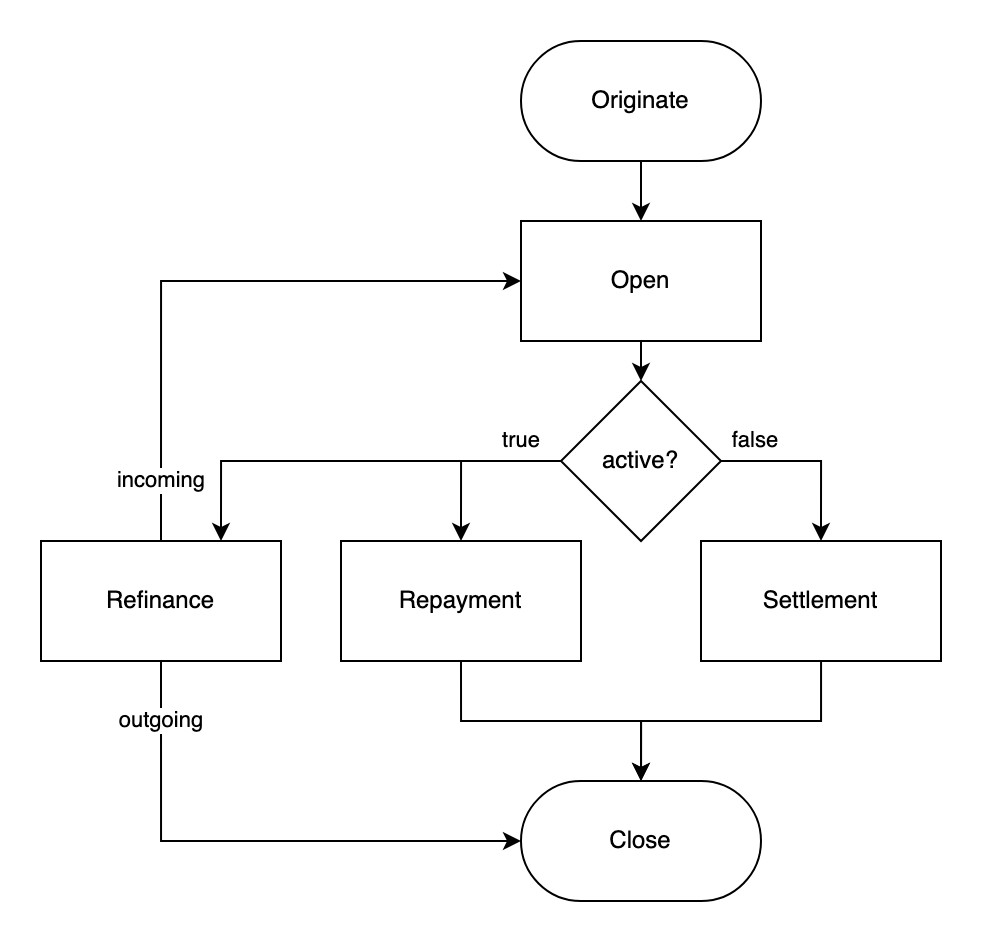
\includegraphics[width=\textwidth]{loan_lifecycle.png}

\begin{itemize}
	\item \textbf{Originate} (action)
	\begin{itemize}
		\item \texttt{Originate} is the action of enforcing conditions in order to create a new loan.

		\item During \texttt{originate}, \texttt{Starport} enforces the transfers of the collateral from the borrower to the \texttt{Custodian}, debt transfers from the lender to the borrower, and enforcing \texttt{additionalTransfers}.\\
			When authentication conditions of the borrower and lender are met, a \texttt{loanId} is created and the state is transitioned to \texttt{Open}.
	\end{itemize}
	
	\item \textbf{Open} (event, condition)
	\begin{itemize}
		\item \texttt{Open} is a state transition by which the loan is created. A \texttt{loanId} is created and stored representing the loan. 
	\end{itemize}
	
	\item \textbf{Active} (condition)
	\begin{itemize}
		\item The \texttt{Status} module provides whether an \texttt{Open} loan is either conditionally active or inactive.\\
			An inactive condition allows a \texttt{Settlement} action to occur. An active condition allows a \texttt{Repayment} action to occur. If the condition flips from active to inactive it is possible for the condition to transition to active again in the future (if a \texttt{Settlement} did not occur).
	\end{itemize}
	
	\item \textbf{Repayment} (action)
	\begin{itemize}
		\item Repayment is the action of a borrower repaying the loan and retrieving their collateral.
		\item The repayment action allows the borrower to repay their loan through the \texttt{Custodian} on the conditions provided by the  \texttt{Pricing} module. During which the lender is repaid. Afterwards, the loan state is transitioned to \texttt{Close}.
	\end{itemize}
	
	\item \textbf{Settlement} (action)
	\begin{itemize}
		\item Settlement is the process of resolving a loan that has transitioned to an inactive status.
		\item Settlement conditions are provided by the \texttt{Settlement} module. The \texttt{Settlement} module returns the authorized fulfiller and conditions of settlement. Specifying the authorized fulfiller is optional. If an authorized fulfiller is not specified any fulfiller can provide the conditions of settlement. Otherwise, settlement is restricted to the authorized fulfiller.
	\end{itemize}
	
	\item \textbf{Refinance} (action)
	\begin{itemize}
		\item \texttt{Refinance} is the action of replacing an existing lender with an incoming lender with no change to the underlying borrower. Refinancing accrues the current debt and the outgoing loan is replaced with an incoming loan.
		\item \texttt{Refinance} conditions are provided by the \texttt{Pricing} module. \texttt{Refinance} enforces transfers from the incoming lender to the existing lender and applies those payments to a new loan and additionally replacing the \texttt{Pricing} parameters. The outgoing loan state is transitioned to \texttt{Close} and an incoming loan state is transitioned to \texttt{Open}.
	\end{itemize}
	
	\item \textbf{Close} (event, condition)
	\begin{itemize}
		\item \texttt{Close} is a state transition by which the loan is deleted. 
		\item A \texttt{Close} event deletes an \texttt{Open} loan by deleting the \texttt{loanId} from storage. A deleted \texttt{loanId} cannot be refinanced, repaid, settled, and cryptographically secured from being originated.
	\end{itemize}
\end{itemize}

\section{Authentication}
There are three methods to ensure the fulfiller is authenticated by the borrower or the lender to transact on their behalf.

\begin{enumerate}
	\item\texttt{msg.sender}
		\begin{itemize}
			\item\texttt{msg.sender} must be equal to either the borrower or lender
		\end{itemize}
    	
	\item approval
		\begin{itemize}
    		\item\texttt{msg.sender} is approved by the either the lender or borrower
    			\begin{itemize}
        			\item approval must be a borrower or lender, it cannot be both
        		\end{itemize}
        \end{itemize}
	\item \texttt{CaveatEnforcer.SignedCaveats}
		\begin{itemize}
    		\item An EIP-712\cite{eip712} signed struct that enforces conditional approval from either the borrower or lender
    			\begin{itemize}
        			\item Validates the signature of the borrower or lender
        			\item Makes an external call to the specified \texttt{CaveatEnforcer} with the signed in data
        		\end{itemize}
        \end{itemize}
\end{enumerate}
\subsection{Origination}
For origination, \texttt{Starport} will ensure that the fulfiller is authenticated by both the borrower and the lender.\\

A fulfiller must provide at least one of the three described authentication methods for both the lender and the borrower.
\subsection{Refinancing}
For refinancing \texttt{Starport} will ensure that the fulfiller is authorized by the refinancing lender.\\

A fulfiller must provide at least one of the three described authentication methods for the lender.

\section{Additional Transfers}
\texttt{additionalTransfers} is a concept within \texttt{originate} that allows the fulfiller to reimburse themselves or other entities in ERC-20, ERC-721, or ERC-1155s for cost incurred to perform the transaction or an additional reward for executing the transaction.\\

\texttt{additionalTransfers} are an array of \texttt{AdditionalTransfer} structs naming the \texttt{from}, \texttt{to}, \texttt{amount}, and token details for a transfer.\\

The fulfiller provides \texttt{additionalTransfers} and the authentication model either allows the transfers or reverts.

\texttt{additionalTransfers} is passed to \texttt{CaveatEnforcer} and validated conditionally. For instance a borrower signs into their \texttt{SignedCaveat} an allowance for an \texttt{additionalTransfer} to reimburse the fulfiller for pre-purchasing an ERC-721.

\section{Representment}
Starport data availability and loan state mutations rely on a concept developed in Astaria v0 called \emph{representment}.\\

\emph{Representment} in a process where all data necessary is stored in memory using a single Solidity \texttt{struct}. The \texttt{struct} is hashed and the resulting hash is stored. An accompanying event is emitted for indexing the \texttt{struct} for later use.\\

\emph{Representment} is a data availability strategy that reduces storage requirements and as an effect reduces transaction gas consumption.\\

When a subsequent call is made to the contracts, the transactor represents the \texttt{struct}. The \texttt{struct} is hashed and the resulting hash is validated against the stored hash before continuing execution.\\

Within Starport the \texttt{Starport.Loan} struct contains all of the values necessary for loan servicing. The \texttt{Starport.Loan} struct is hashed using \texttt{keccak256} into a single \texttt{bytes32} value \texttt{loanId}.
Any subsequent call to Starport or modules requires the \texttt{Starport.Loan} struct be represented, and validated as an \texttt{Open} loan.


\begin{thebibliography}{9}
\bibitem{erc20}
Fabian Vogelsteller, Vitalik Buterin. 
\textit{ERC-20: Token Standard}. 
Ethereum Improvement Proposals, 2015.\\
https://eips.ethereum.org/EIPS/eip-20

\bibitem{erc721}
 William Entriken, Dieter Shirley, Jacob Evans, Nastassia Sachs. 
\textit{ERC-721: Non-Fungible Token Standard}. 
Ethereum Improvement Proposals, 2018.\\
https://eips.ethereum.org/EIPS/eip-721

\bibitem{erc1155}
Witek Radomski, Andrew Cooke, Philippe Castonguay, James Therien, Eric Binet, Ronan Sandford. 
\textit{ERC-1155: Multi Token Standard}. 
Ethereum Improvement Proposals, 2018.\\
https://eips.ethereum.org/EIPS/eip-1155

\bibitem{eip712}
Remco Bloemen, Leonid Logvinov, Jacob Evans.
\textit{EIP-712: Typed structured data hashing and signing} 
Ethereum Improvement Proposals, 2017.\\
https://eips.ethereum.org/EIPS/eip-712

% Add more references as needed
\end{thebibliography}

\end{document}
